

% The actual figure file is inside common-files/Figs/. Therefore, 
% when this file is inclucded in another tex file located in folder A, 
% a symbolic link should be created inside A/Figs to link the filename
% to the actual figure file inside the common-files/Figs/ folder.
\begin{figure}[htb]
  \begin{center}
    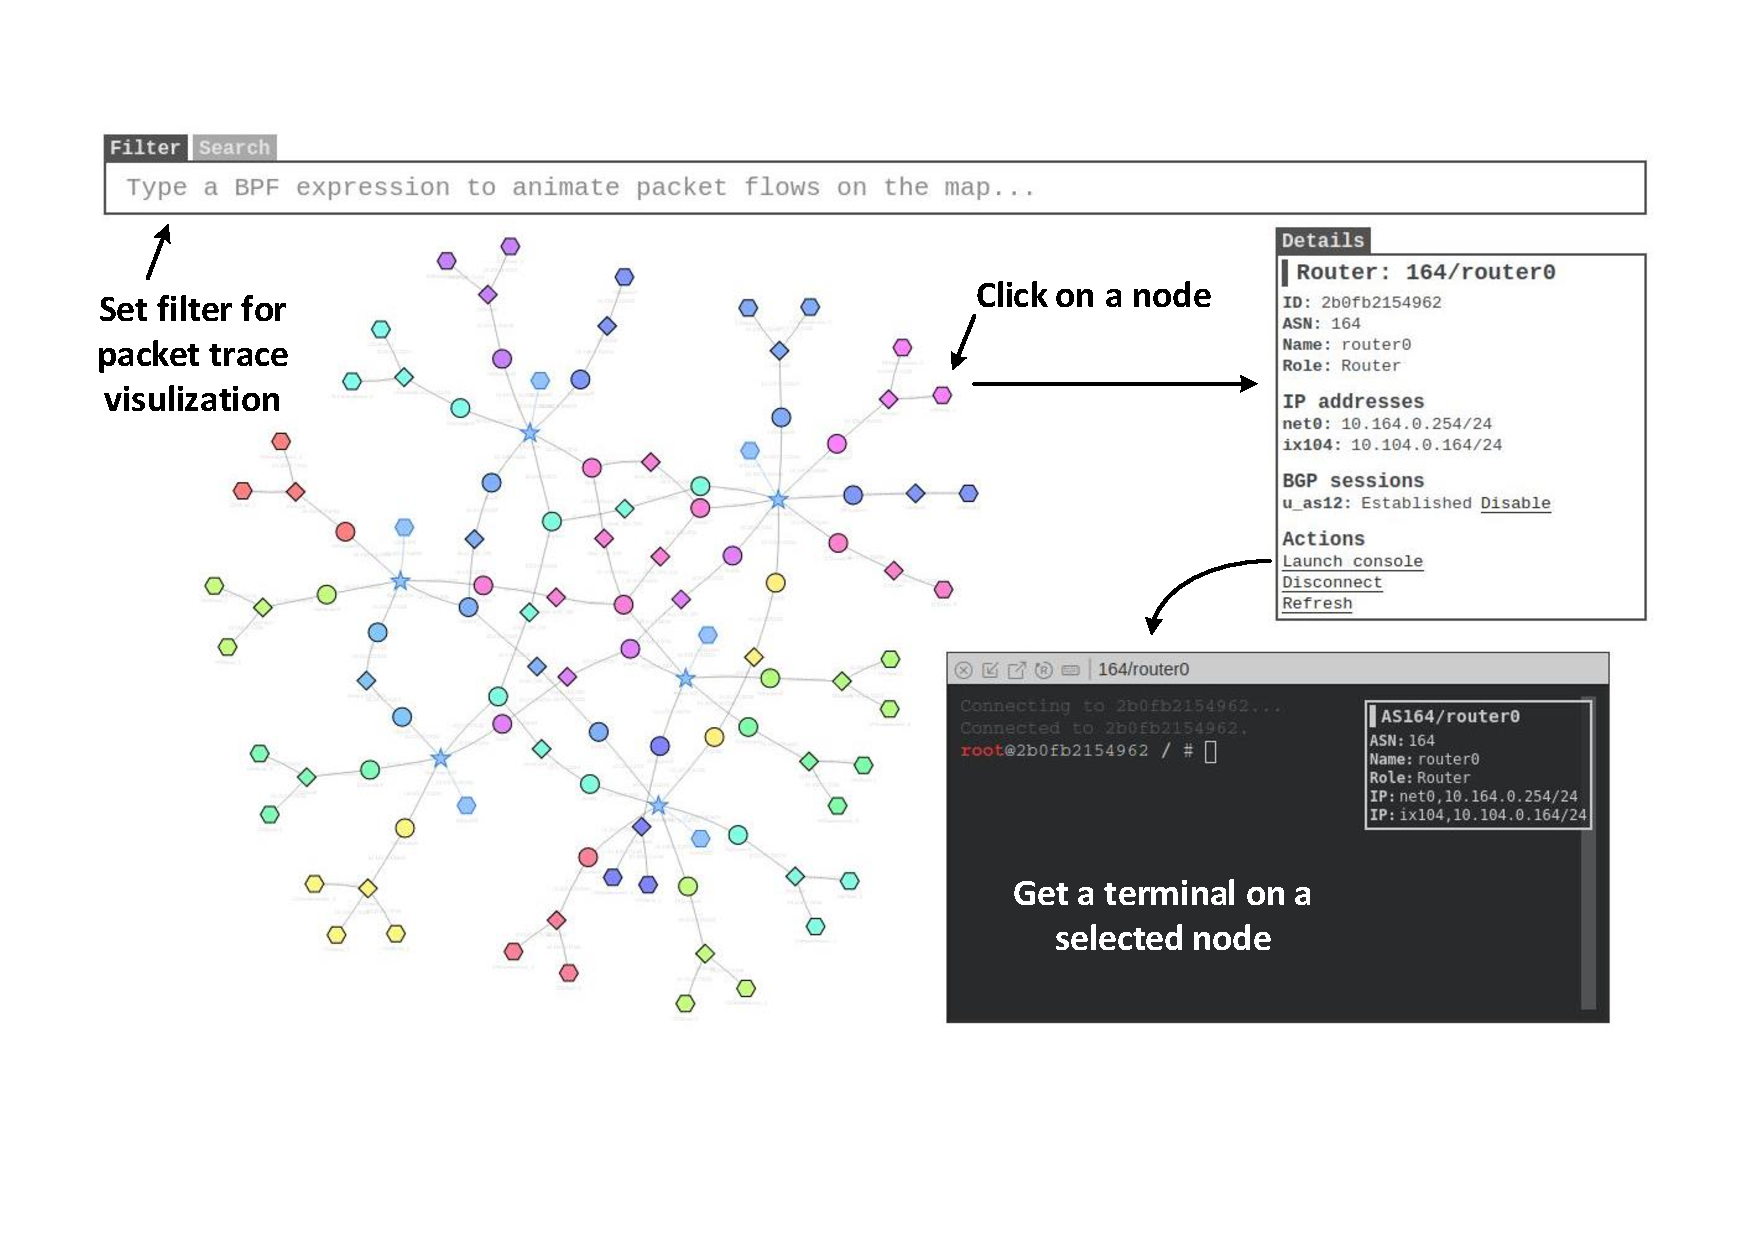
\includegraphics[width=0.95\textwidth]{./Figs/emulator_gui.pdf}
  \end{center}
  \caption{The map of the emulated Internet}
  \label{emulator:fig:emulator-gui}
\end{figure}


Each computer (hosts or routers) running inside the emulator is a docker container.
Users can access these computers using docker commands, such as getting a shell
inside a container.
The emulator also comes with a web application, which visualizes all the hosts, routers,
and networks.
After the emulator starts, the map can be accessed from this
URL: \url{http://localhost:8080/map.html}.
See Figure~\ref{emulator:fig:emulator-gui}.
To zoom in/out, use the mouse middle scroll. 
Click on any node, the detailed information of that node
will be displayed on the side panel, from where,
users can get a console on that node (container). 




